\section{Auswertung}
\label{sec:Auswertung}




%%%%%%%%%%%%%%%%%%%%%%%%%%%%%%%%%%%%%%%%%%%%%%%%%%%%%%%%%%%%%%%%%%%%%%%%%%%%%%%%%%%%%%%%%%%%%%
% Teil a)
\subsection{Ermittlung der Grenzfrequenzen aus Durchlasskurven}

\subsubsection{Durchlasskurve der LC-Kette}
\label{sec:durchLC}
Der theoretische Wert für die Grenzfrequenz $f_{\text{G}}$ ergibt sich nach Formel \eqref{eqn:wgrenz_lc} zu
\begin{equation}
	f_{\text{G}} = \frac{1}{\pi \sqrt{LC}} \text{.}
\end{equation}
Man erhält nach Einsetzen der Bauteilgrößen für die theoretische Grenzfrequenz
\begin{equation*}
	f_{\text{G}} = \SI{64310.7}{\hertz} \, \text{.}
\end{equation*}

Die mit dem X-Y-Schreiber aufgezeichnete Durchlasskurve für die LC-Kette ist in Abbildung
\ref{fig:durchiLC} zu sehen.
\begin{figure}
	\centering
	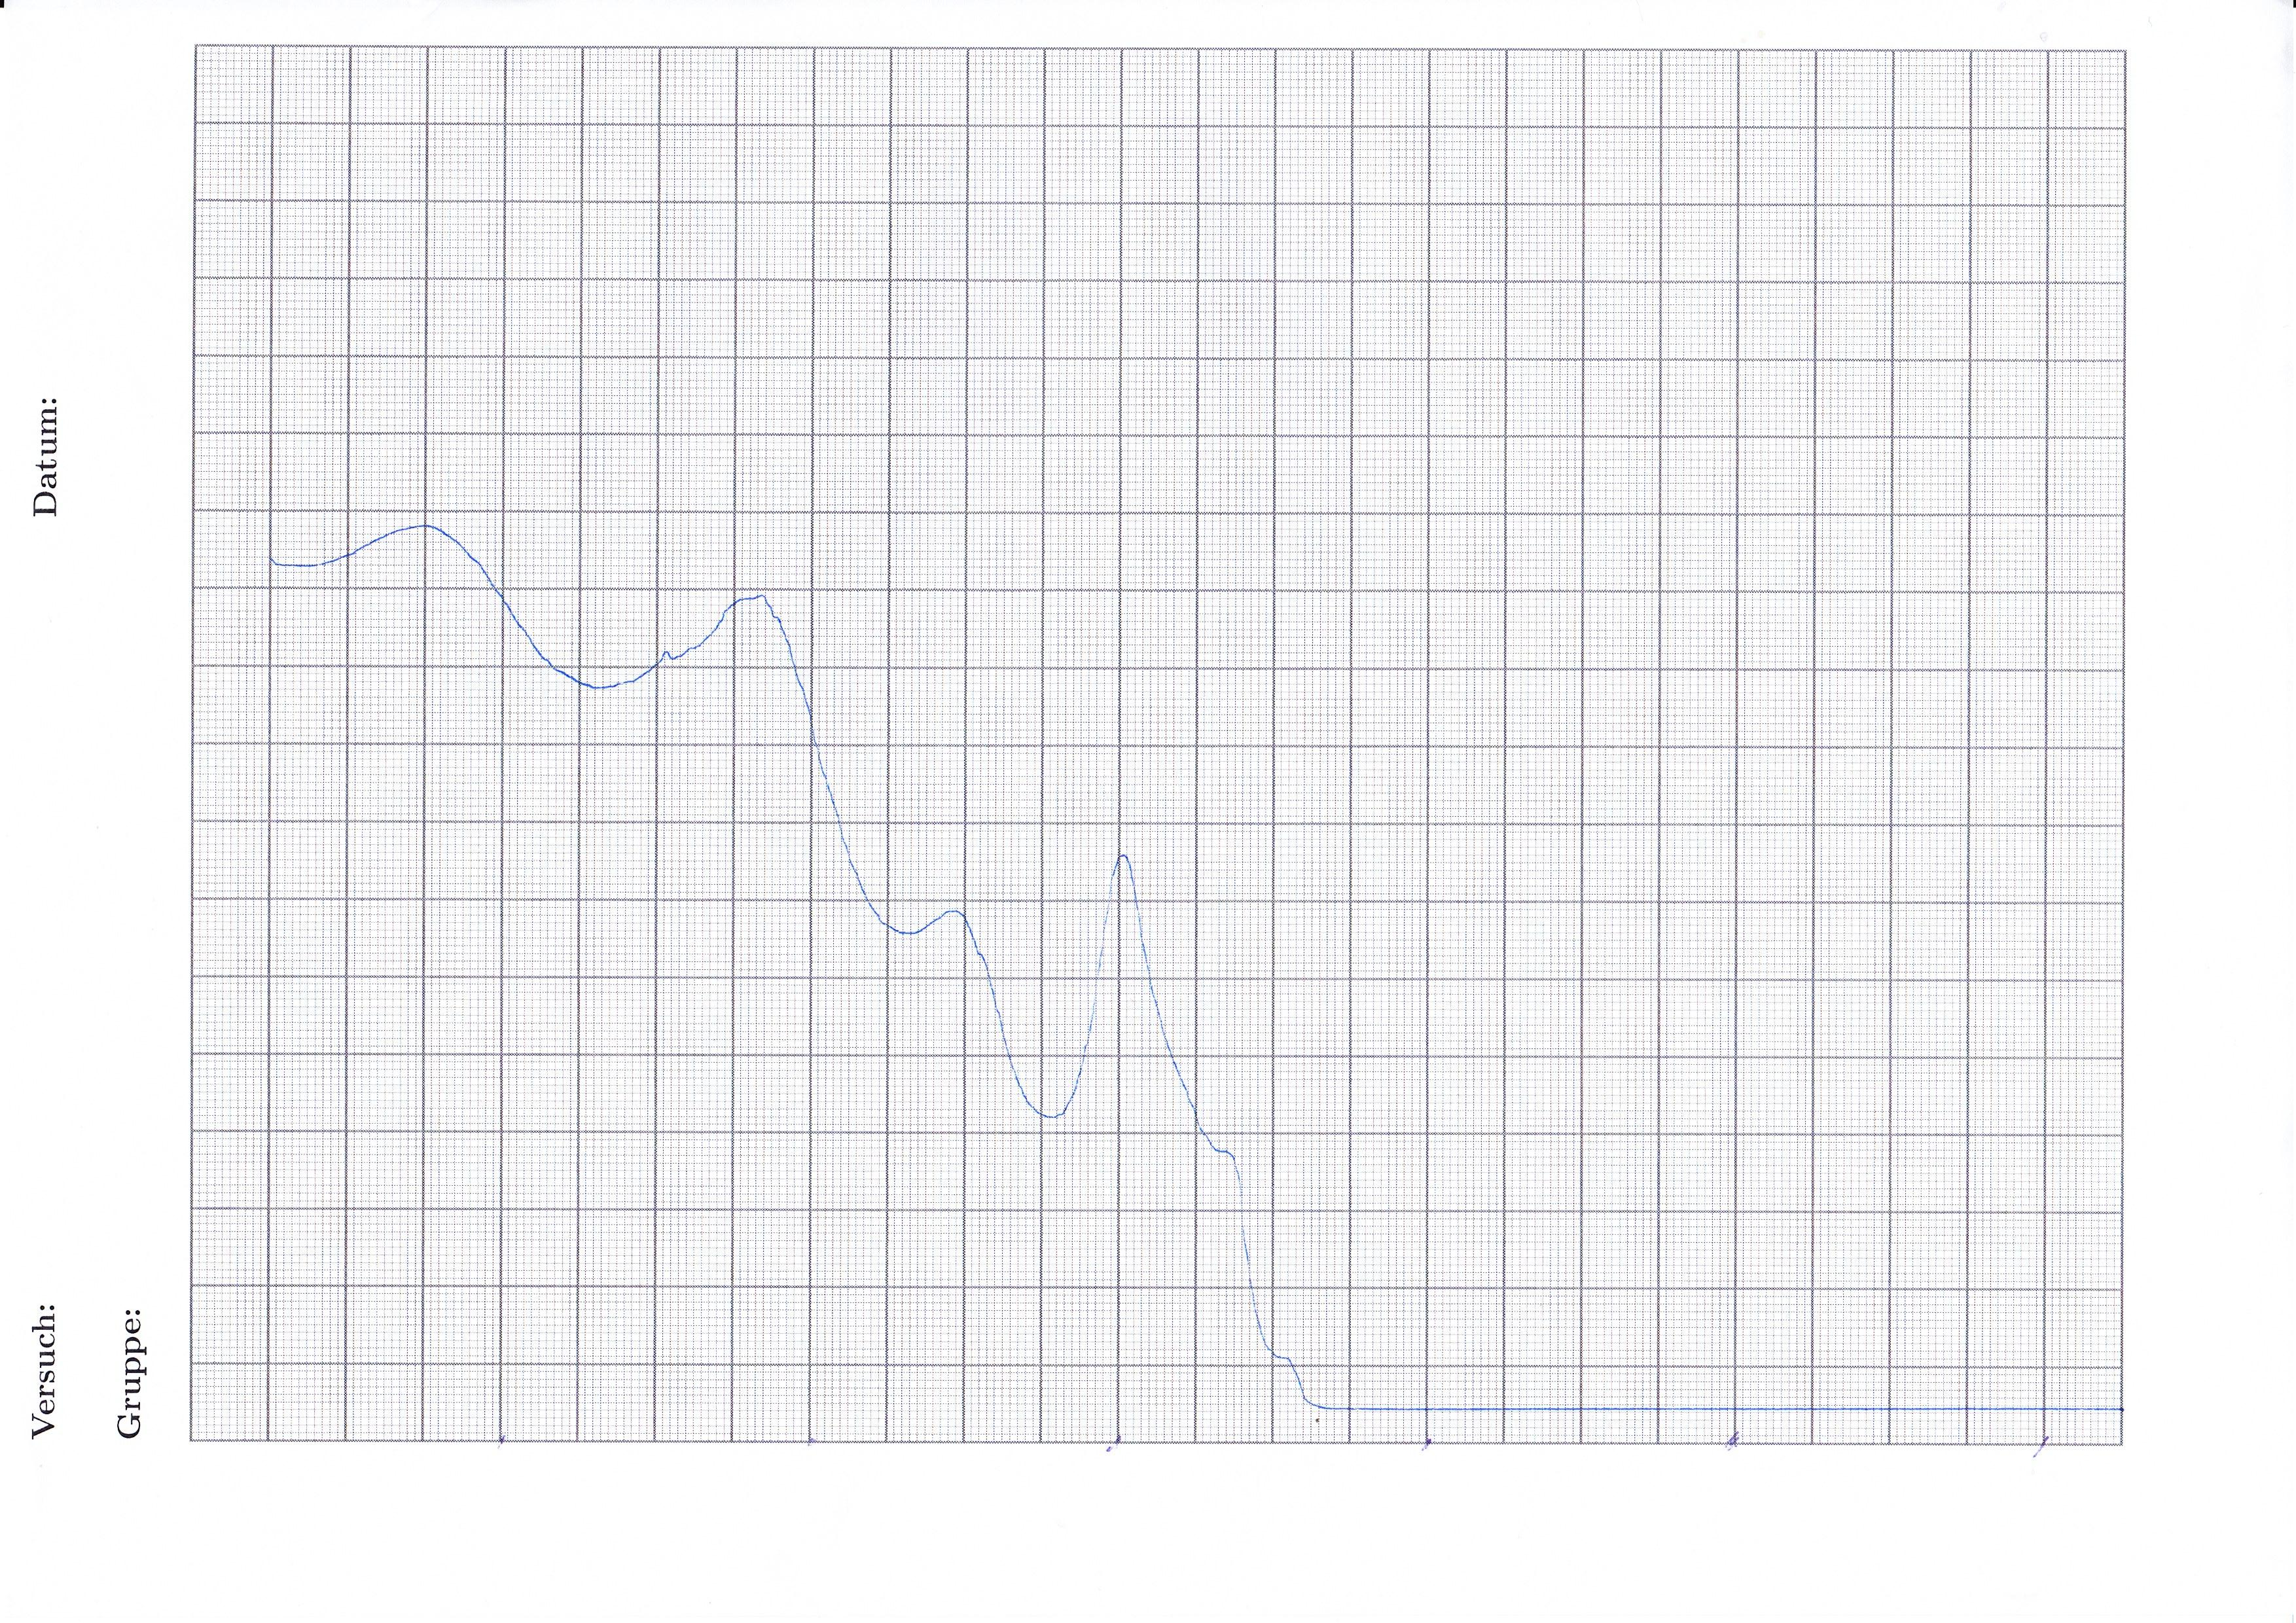
\includegraphics[width=1.02\textwidth]{Bilder/durchlasskurve_lc_kette.jpg}
	\caption{Durchlasskurve der LC-Kette: Ausgangsspannung $U_{\text{aus}}$ gegen die
		Frequenz $\omega$ aufgetragen.}
	\label{fig:durchiLC}
\end{figure}
Die Referenzpunkte für die Skalarierung des Millimeterpapiers sind in Tabelle
\ref{tab:skalaLC} aufgetragen. Hierbei entsprechen die $x$-Werte der horizontalen Position
auf dem Millimeterpapier und die Frequenzen $f$ der zu diesem Zeitpunkt abgelesenen Frequenz.

\begin{table}
	\caption{Messdaten zur Skalierung der $x$-Achse des Millimeterpapiers bei der
	Durchlasskurve der LC-Kette.}
	\label{tab:skalaLC}
	\centering
	\begin{tabular}{cc}
		\toprule
		$x$/$\si{\centi\meter}$ & $f$/$\si{\kilo\hertz}$ \\
		\midrule
		4.0                     & 37.72                  \\
		8.0                     & 45.22                  \\
		12.0                    & 56.25                  \\
		16.0                    & 67.84                  \\
		20.0                    & 84.24                  \\
		24.0                    & 105.80                 \\
		\bottomrule
	\end{tabular}
\end{table}
Aus den Messdaten in Tabelle \ref{tab:skalaLC} wird nun aufgrund der logarithmischen
Abhängigkeit von $x$ von der Frequenz $f$ eine Ausgleichsrechnung mit der Funktion
$f(x) = a \cdot \mathrm{e}^{bx}$ durchgeführt.
Für die Paramter erhält man:
\begin{gather*}
	a = (29,79 \pm 0,55) \, \si{\kilo\hertz} \, \text{,}  \\
	b = (0,0525 \pm 0,0010) \, \si{\centi\meter} \text{.}
\end{gather*}
Damit ergibt sich die Skalierung der $x$-Achse zu
\begin{equation}
	f(x) = a \cdot \mathrm{e}^{bx} \text{,}
\end{equation}
mit den Parametern oben.

Aus der Durchlasskurve in Abbildung \ref{fig:durchiLC} lässt sich die $x$-Position mit einem
Ablesefehler zu $x_{\text{G}} = (14,6 \pm 0,1) \, \si{\centi\meter}$ bestimmen.
Damit erhält man für die Grenzfrequenz mit Gaußscher Fehlerfortpflanzung (Formel
\eqref{eqn:fehlerfortpflanzung}):
%%%%%%%%%%%%%%%%%%%%%%%%%%%%%%%%


%z.B.
%Damit erhält man für die Grenzfrequenz mittels einer Regression von f(x) mit python/matplotlib \cite{matplotlib}



%%%%%%%%%%%%%%%%%%%%%%%%%%%%%%%%
\begin{equation*}
	f_{\text{G}} = (64,115 \pm 1,546 ) \, \si{\kilo\hertz} \text{.}
\end{equation*}


\FloatBarrier
\subsubsection{Durchlasskurve der LC$_1$C$_2$-Kette}

Die theoretischen Grenzfrequenzen für die LC$_1$C$_2$-Kette mit den Werten für
$L$, $C_1$ und $C_2$ ergeben sich zu:
\begin{gather*}
	f_0 = \frac{1}{2\pi} \sqrt{\frac{2}{LC_1}} = \SI{45475}{\hertz} \text{,} \\
	f_1 = \frac{1}{2\pi} \sqrt{\frac{2}{LC_2}} = \SI{66511}{\hertz} \text{,} \\
	f_2 = \frac{1}{2\pi} \sqrt{\frac{2}{L} \frac{C_1+C_2}{C_1C_2}} = \SI{80571}{\hertz} \text{.}
\end{gather*}

Die Durchlasskurve der LC$_1$C$_2$-Kette ist in Abbildung \ref{fig:durchiLCC} dargestellt.

\begin{figure}
	\centering
	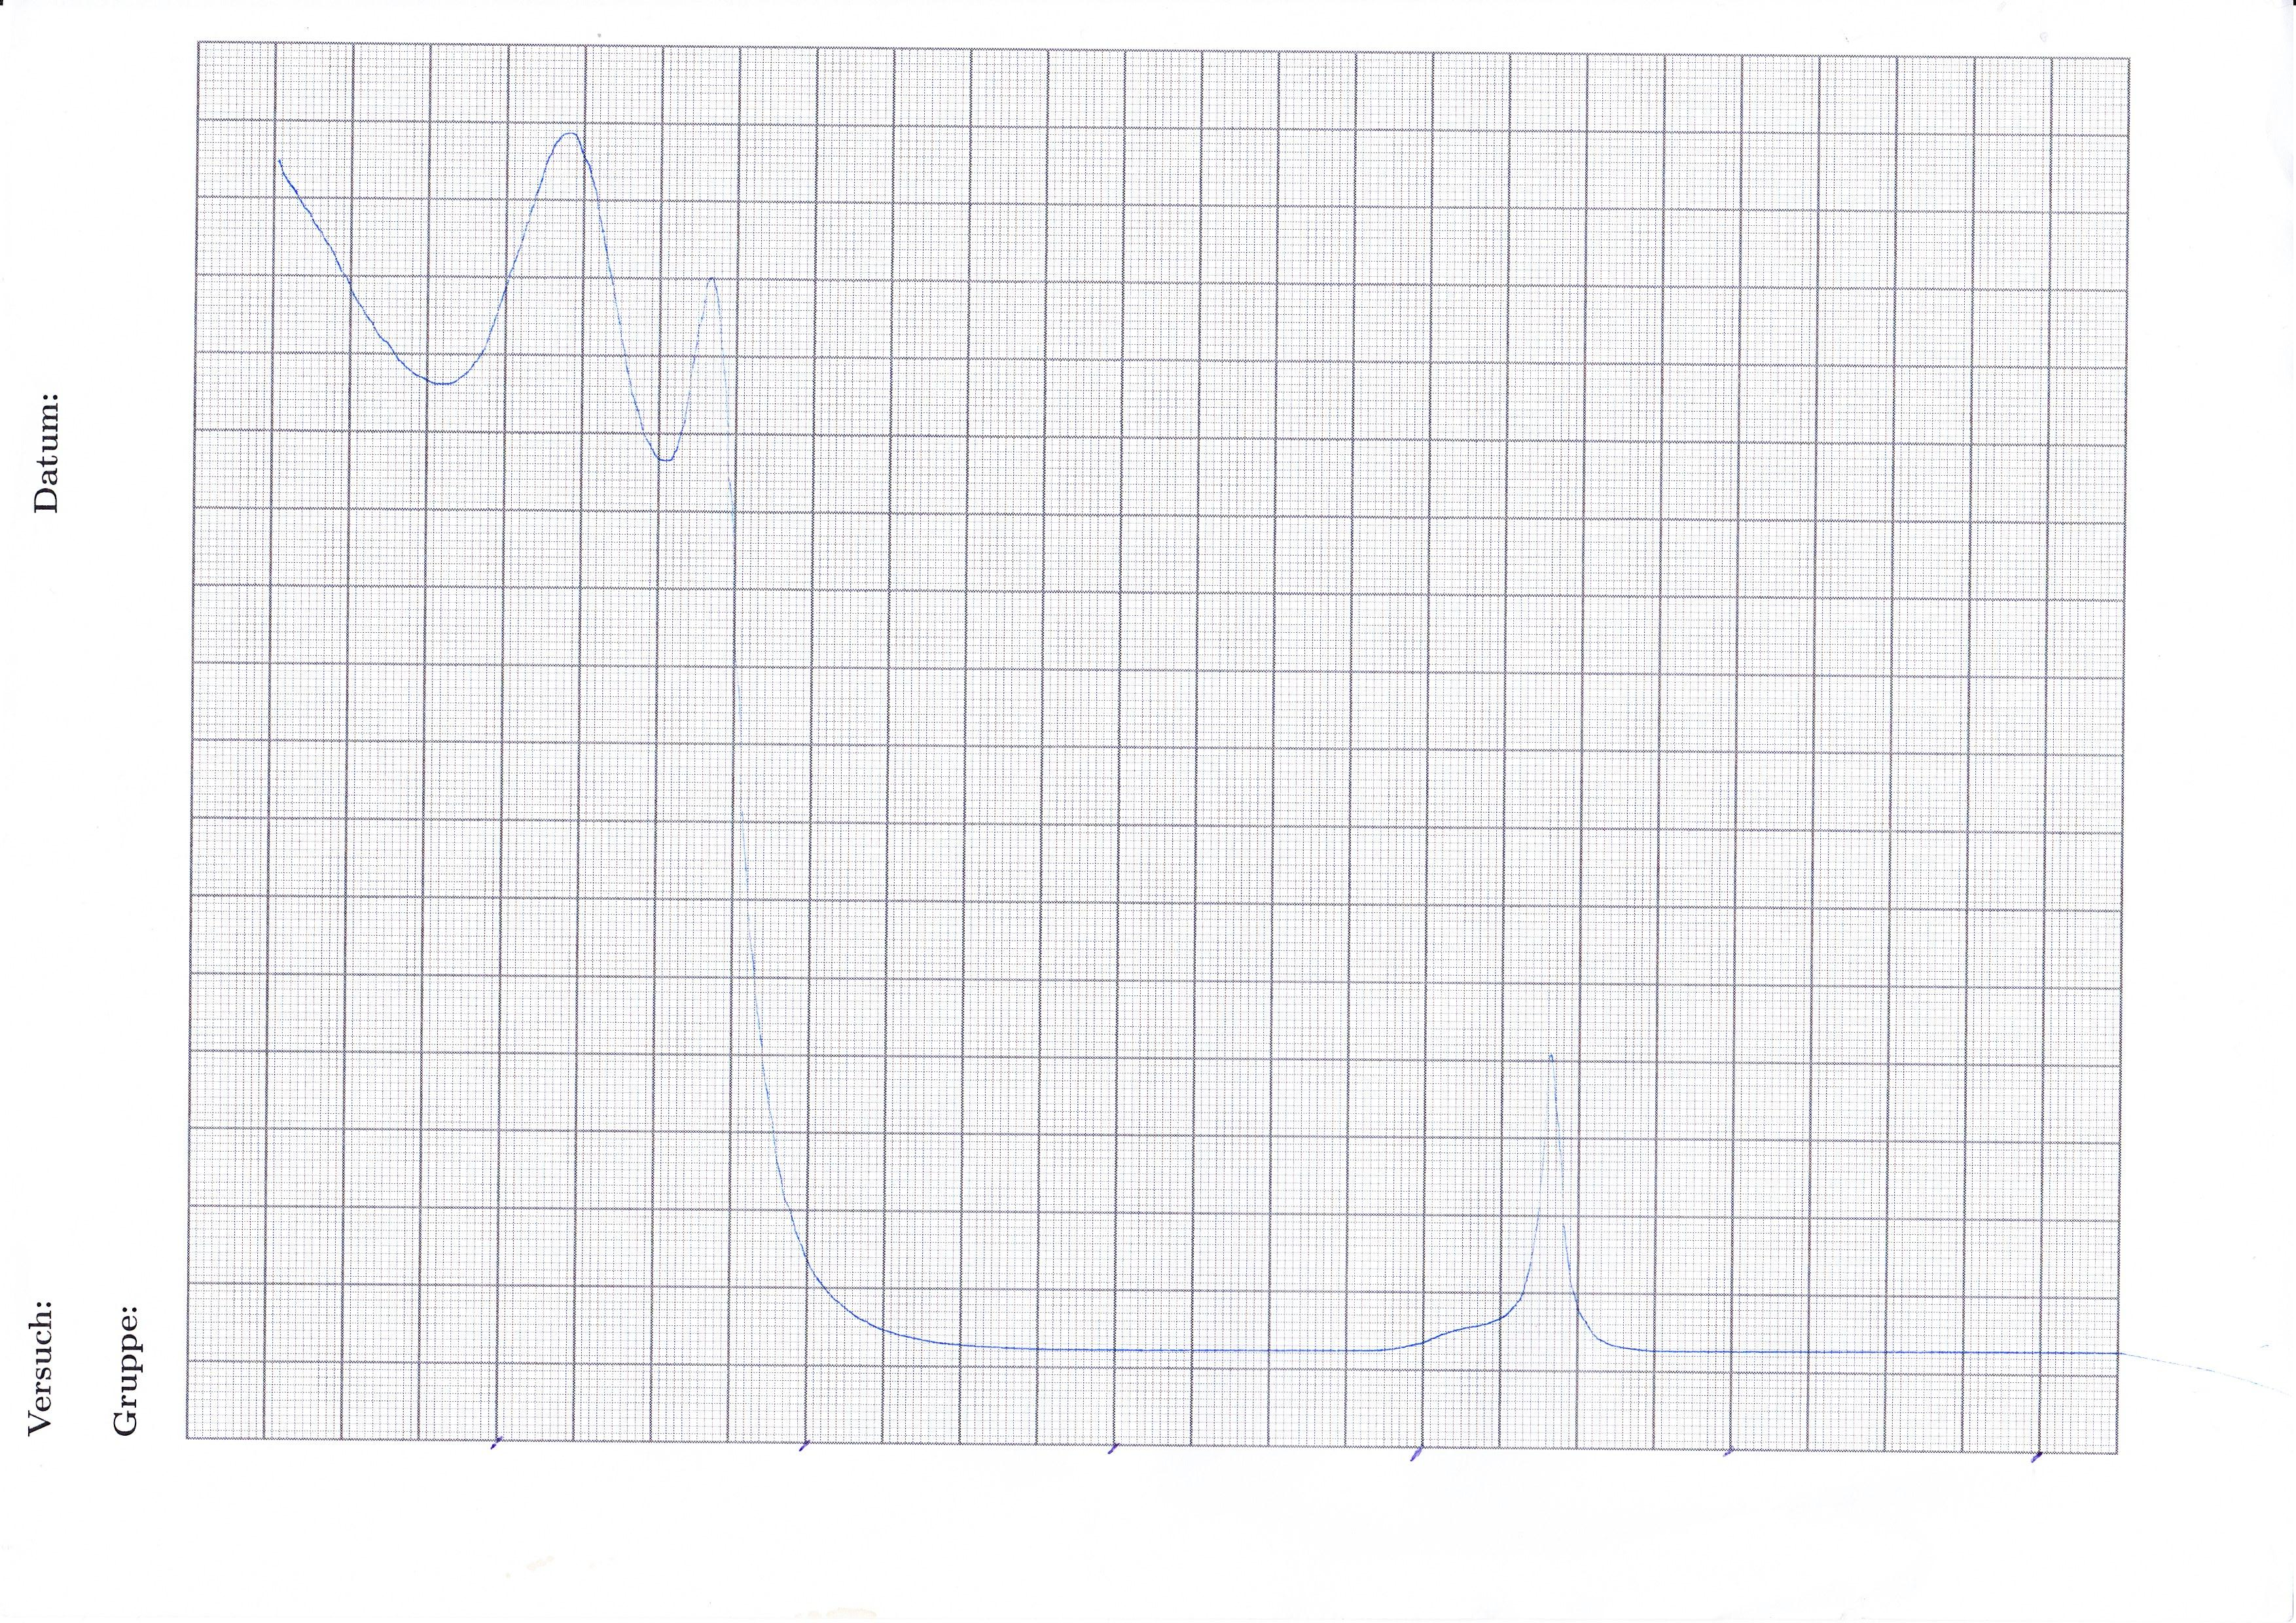
\includegraphics[width=1.02\textwidth]{Bilder/durchlasskurve_lc1c2.jpg}
	\caption{Durchlasskurve der LC$_1$C$_2$-Kette: Ausgangsspannung $U_{\text{aus}}$ gegen
		die Frequenz $\omega$ aufgetragen.}
	\label{fig:durchiLCC}
\end{figure}

Die Messwerte für die Referenzpunkte zur Skalarierung der $x$-Achse sind in Tabelle
\ref{tab:skalaLCC} aufgetragen.

\begin{table}
	\caption{Messdaten zur Skalierung der $x$-Achse des Millimeterpapiers bei der
	Durchlasskurve der LC$_1$C$_2$-Kette.}
	\label{tab:skalaLCC}
	\centering
	\begin{tabular}{cc}
		\toprule
		$x$/$\si{\centi\meter}$ & $f$/$\si{\kilo\hertz}$ \\
		\midrule
		4.0                     & 36.50                  \\
		8.0                     & 45.15                  \\
		12.0                    & 56.60                  \\
		16.0                    & 68.21                  \\
		20.0                    & 82.77                  \\
		24.0                    & 105.48                 \\
		\bottomrule
	\end{tabular}
\end{table}
Analog wie in Abschnitt \ref{sec:durchLC} ergeben sich die Paramater der Ausgleichsfunktion
\begin{equation*}
	f(x) = a \cdot \mathrm{e}^{bx}
\end{equation*}
zu
\begin{gather*}
	a = (29,56 \pm 0,68) \, \si{\kilo\hertz} \text{,} \\
	b = (0,0525 \pm 0,0012) \, \si{\centi\meter} \text{.}
\end{gather*}
Die Positionen $x_\text{n}$ der Grenzfrequenzen lassen sich aus Abbildung \ref{fig:durchiLCC}
ablesen, man erhält:
\begin{gather*}
	x_0 = (10,8 \pm 0,1) \, \si{\centi\meter} \, \text{,} \\
	x_1 = (15,5 \pm 0,1) \, \si{\centi\meter} \, \text{,} \\
	x_2 = (18,9 \pm 0,1) \, \si{\centi\meter} \, \text{.}
\end{gather*}

Mittels der Skalierungsfunktion, den bestimmten Paramatern und Gaußscher Fehlerfortpflanzung
%%%%%%%%%%%%%%%%%%
%einer Ausgleichsrechnung mittels python/matplotlib \cite{matplotlib}
%%%%%%%%%%%%%%%%%%%%%%%%%
(Formel \eqref{eqn:fehlerfortpflanzung}) erhält man nun die drei Grenzfrequenzen der
LC$_1$C$_2$-Kette zu:
\begin{gather*}
	f_0 = (52,170 \pm 1,405) \, \si{\kilo\hertz} \, \text{,} \\
	f_1 = (66,801 \pm 2,007) \, \si{\kilo\hertz} \, \text{,} \\
	f_2 = (79,883 \pm 2,615) \, \si{\kilo\hertz} \, \text{.}
\end{gather*}

%%%%%%%%%%%%%%%%%%%%%%%%%%%%%%%%%%%%%%%%%%%%%%%%%%%%%%%%%%%%%%%%%%%%%%%%%%%%%%%%%%%%%%%%%%%%%%
% Teil b)
\FloatBarrier
\subsection{Dispersionskurven nach Dispersionsrelation}

\subsubsection{Dispersionskurve der LC-Kette}
Die Dispersionskurve ergibt sich nach Gleichung \eqref{eqn:dispersion} mit
\begin{equation}
	\label{eqn:dispisi}
	\omega = \sqrt{\frac{2}{LC}(1-\cos\theta)} \, \text{,}
\end{equation}
da negative Frequenzen nicht betrachtet werden.
Die Phasenverschiebung pro Kettenglied $\theta$ ergibt sich durch
\begin{equation}
	\theta = \frac{\phi}{n} \, \text{,}
\end{equation}
wobei $\phi$ der gemessenen Phasenverschiebung zwischen Eingangsspannung $U_{\text{ein}}$
und Ausgangsspannung $U_{\text{aus}}$ entspricht.

Die sich ergebenden Werte sind in Tabelle \ref{tab:dispersionlc} aufgetragen.

\begin{table}
	\caption{Messdaten zur Untersuchung der Dispersionskurve einer LC-Kette.}
	\label{tab:dispersionlc}
	\centering
	\begin{tabular}{cccc}
		\toprule
		$\phi$/$\si{\radian}$ & $f$/$\si{\kilo\Hz}$ & $\omega$/$\si{\kilo\Hz}$ & $\theta$/$\si{\radian}$ \\
		\midrule
		$\pi$                 & 7.2                 & 45.2                     & 0.22                    \\
		2$\pi$                & 14.3                & 89.8                     & 0.45                    \\
		3$\pi$                & 21.4                & 134.5                    & 0.67                    \\
		4$\pi$                & 28.3                & 177.8                    & 0.90                    \\
		5$\pi$                & 34.7                & 218.0                    & 1.12                    \\
		6$\pi$                & 41.0                & 257.6                    & 1.35                    \\
		7$\pi$                & 46.4                & 291.5                    & 1.57                    \\
		8$\pi$                & 51.5                & 323.6                    & 1.80                    \\
		9$\pi$                & 56.0                & 351.9                    & 2.02                    \\
		10$\pi$               & 58.7                & 368.8                    & 2.24                    \\
		11$\pi$               & 61.1                & 383.9                    & 2.47                    \\
		12$\pi$               & 63.2                & 397.1                    & 2.69                    \\
		13$\pi$               & 64.4                & 404.6                    & 2.92                    \\
		\bottomrule
	\end{tabular}
\end{table}

Die theoretische Dispersionskurve nach Gleichung \eqref{eqn:dispisi} mit den zugehörigen
Messwerten ist in Abbildung \ref{fig:dispilc} dargestellt.

\begin{figure}
	\centering
	\includegraphics{Bilder/b1.pdf}
	\caption{Dispersionskurve der LC-Kette: Kreisfrequenz $\omega$ gegen die Phasenverschiebung pro Kettenglied $\theta$ aufgetragen.}
	\label{fig:dispilc}
\end{figure}

\FloatBarrier
\subsubsection{Dispersionskurve der LC$_1$C$_2$-Kette}
Die Dispersionskurve für die LC$_1$C$_2$-Kette ergibt sich nach Formel \eqref{eqn:dispersion2}.

Analog wie bei der LC-Kette erhält man die Messdaten, die in Tabelle \ref{tab:dispersioncc}
aufgetragen sind.

\begin{table}
	\caption{Messdaten zur Untersuchung der Dispersionskurve einer LC$_1$C$_2$-Kette.}
	\label{tab:dispersioncc}
	\centering
	\begin{tabular}{cccc}
		\toprule
		$\phi$/$\si{\radian}$ & $f$/$\si{\kilo\Hz}$ & $\omega$/$\si{\kilo\Hz}$ & $\theta$/$\si{\radian}$ \\
		\midrule
		$\pi$                 & 8.65                & 54.3                     & 0.22                    \\
		2$\pi$                & 17.05               & 107.1                    & 0.45                    \\
		3$\pi$                & 25.10               & 157.7                    & 0.67                    \\
		4$\pi$                & 32.45               & 203.9                    & 0.90                    \\
		5$\pi$                & 38.90               & 244.4                    & 1.12                    \\
		6$\pi$                & 43.80               & 275.2                    & 1.35                    \\
		7$\pi$                & 73.80               & 463.7                    & 1.57                    \\
		8$\pi$                & 75.10               & 471.9                    & 1.80                    \\
		\bottomrule
	\end{tabular}
\end{table}

Die theoretische Dispersionskurve nach Gleichung \eqref{eqn:dispersion2} mit den zugehörigen Messwerten ist in Abbildung \ref{fig:dispicc} dargestellt.

\begin{figure}
	\centering
	\includegraphics{Bilder/b2.pdf}
	\caption{Dispersionskurve der LC$_1$C$_2$-Kette: Kreisfrequenz $\omega$ gegen die Phasenverschiebung pro Kettenglied $\theta$ aufgetragen.}
	\label{fig:dispicc}
\end{figure}



%%%%%%%%%%%%%%%%%%%%%%%%%%%%%%%%%%%%%%%%%%%%%%%%%%%%%%%%%%%%%%%%%%%%%%%%%%%%%%%%%%%%%%%%%%%%%%
%c
\FloatBarrier
\subsection{Phasengeschwindigkeit in einer $LC$-Kette}

Aus den bestimmten Eigenfrequenzen $f$ der $LC$-Kette und den zugehörigen Phasenverschiebungen $\theta$ lassen sich nach Formel \eqref{eqn:v-phase} die jeweiligen Phasengeschwindigkeiten berechnen.\\
Die Theoriekurve ergibt sich ebenso nach Formel \eqref{eqn:v-phase}.\\
$\theta$, also die Phasenverschiebung pro Kettenglied, ergibt sich aus der Phasenverschiebung $\phi$ über die gesamte $LC$-Kette dividiert durch die Anzahl der Kettenglieder $n=14$.\\
In Tabelle \ref{tab:c} finden sich die Nummern der Entartungen $n$ der Lissajou-Figuren zu Geraden, welche der Phasenverschiebung $\phi$ über der gesamten $LC$-Kette mit $\phi=n\pi$ entsprechen samt den zugehörigen Eigenfrequenzen $f$.\\
Zudem werden die Eigenfrequenzen umgerechnet in die Kreisfrequenz $\omega$ und die Phasenverschiebung pro Kettenglied $\theta$ in die Tabelle eingetragen. \\
In der fünften Spalte findet sich die Phasengeschwindigkeit nach $v_{\mathrm{Ph}}=\frac{\omega}{\theta}$.

In Abbildung \ref{fig:plotc} sind die gefundenden Messwerte der Phasengeschwindigkeit im Vergleich zur Theoriekurve aufgetragen.
\begin{table}
	\caption{Phasengeschwindigkeiten zu den jeweiligen Eigenfrequenzen der $LC$-Kette.}
	\label{tab:c}
	\centering
	\begin{tabular}{ccccc}
		\toprule
		Phasenverschiebung $\phi$/$\pi\si{\radian}$ & $f$/$\si{\kilo\Hz}$ & $\omega$/$\si{\kilo\Hz}$ & $\theta$/$\si{\radian}$ & $v_{\mathrm{Ph}}$/\si{\kilo\metre\per\second} \\
		\midrule
		1.0                                         & 7.2                 & 45.2                     & 0.22                    & 201.6                                         \\
		2.0                                         & 14.3                & 89.8                     & 0.45                    & 200.2                                         \\
		3.0                                         & 21.4                & 134.5                    & 0.67                    & 199.73                                        \\
		4.0                                         & 28.3                & 177.8                    & 0.9                     & 198.1                                         \\
		5.0                                         & 34.7                & 218.0                    & 1.12                    & 194.32                                        \\
		6.0                                         & 41.0                & 257.6                    & 1.35                    & 191.33                                        \\
		7.0                                         & 46.4                & 291.5                    & 1.57                    & 185.6                                         \\
		8.0                                         & 51.5                & 323.6                    & 1.8                     & 180.25                                        \\
		9.0                                         & 56.0                & 351.9                    & 2.02                    & 174.22                                        \\
		10.0                                        & 58.7                & 368.8                    & 2.24                    & 164.36                                        \\
		11.0                                        & 61.1                & 383.9                    & 2.47                    & 155.53                                        \\
		12.0                                        & 63.2                & 397.1                    & 2.69                    & 147.47                                        \\
		13.0                                        & 64.4                & 404.6                    & 2.92                    & 138.71                                        \\
		\bottomrule
	\end{tabular}
\end{table}
\begin{figure}
	\centering
	\includegraphics{Bilder/c.pdf}
	\caption{Phasengeschwindigkeit der $LC$-Kette an jedem Kettenglied aufgetragen gegen die Kreisfrequenz.}
	\label{fig:plotc}
\end{figure}
%%%%%%%%%%%%%%%%%%%%%%%%%%
%d
\FloatBarrier
\subsection{Spannungsverlauf der $LC$-Kette bei offenem Ende}
Die gemessenen Spannungsamplituden an jedem Kettenglied bei der 1. und 2. Eigenschwingung der $LC$-Kette finden sich in Tabelle \ref{tab:ei}.

\begin{table}
	\centering
	\caption{Messwerte der Spannungsamplitude an jedem $LC$-Kettenglied für die ersten beiden Eigenschwingungen.}
	\label{tab:ei}
	\begin{tabular}{ccc}
		\toprule
		Nummer des Kettenglieds & $U$/$\si{\volt}$ bei 1.Eigenschwingung & $U$/$\si{\volt}$ bei 2.Eigenschwingung \\
		\midrule
		0                       & 0.93                                   & 1.11                                   \\
		1                       & 1.17                                   & 0.81                                   \\
		2                       & 1.2                                    & 0.3                                    \\
		3                       & 1.14                                   & 0.07                                   \\
		4                       & 0.84                                   & 0.35                                   \\
		5                       & 0.63                                   & 0.6                                    \\
		6                       & 0.3                                    & 0.69                                   \\
		7                       & 0.09                                   & 0.78                                   \\
		8                       & 0.225                                  & 0.6                                    \\
		9                       & 0.65                                   & 0.3                                    \\
		10                      & 0.84                                   & 0.15                                   \\
		11                      & 0.75                                   & 0.66                                   \\
		12                      & 0.78                                   & 1.05                                   \\
		13                      & 0.9                                    & 1.05                                   \\
		\bottomrule
	\end{tabular}
\end{table}

Die Grundschwingung, also die erste Eigenschwingung der $LC$-Kette, betrug $w_{\mathrm{0}}=7.5 \,\si{\kilo\Hz}$, die erste Oberschwingung, also die 2. Eigenschwingung betrug $w_{\mathrm{1}}=14.7 \,\si{\kilo\Hz}$.

Nach Formel  \eqref{eqn:abschluss} wird bei der beidseitig offenen $LC$-Kette, also $R=\infty$ an den Enden der LC-Kette ein Maximum der Spannungsamplitude angenommen, sowie kein Phasensprung am Kettenende erwartet.

In Abbildung \ref{fig:plotdeins} sind die jeweilig gemessenen Spannungsamplituden bei den ersten beiden Eigenschwingungen gegen die Nummer der Kettenglieder aufgetragen.

Der erwartete Spannungsverlauf einer stehenden Cosinus-Welle wird durch die Messdaten annähernd erreicht. Die stehende Welle weist bei der Grundschwingung einen Spannungsknoten etwa in der Mitte der $LC$-Kette auf, während an den Enden Spannungsbäuche auftreten.
Daher findet auch wie erwartet kein Phasensprung am Kettenende statt.
Der Spannungsverlauf bei der ersten Eigenschwingung bildet sich eine stehende Welle mit halber Wellenlänge.

In Abbildung \ref{fig:plotd} zeigt sich ebenso der erwarteten Verlauf der Spannungsamplituden für die zweite Eigenschwingung.\\
Erneut zeigen sich an Anfang und Ende der $LC$-Kette Spanungsbäuche, es findet also wieder wie erwartet kein Phasensprung am Kettenende statt.
Etwa in der Mitte der $LC$-Kette zeigt sich ein dritter Wellenbauch und es ergeben sich somit 2 Schwingungsknoten und 3 Schwingungsbäuche.
Die erste Oberschwingung weist somit genau eine Wellenlänge auf.
\begin{figure}
	\centering
	\includegraphics{Bilder/d.pdf}
	\caption{Spannungsverlauf der offenen $LC$-Kette für $f=7.5 \,\si{\kilo\Hz}$(Grundschwingung).}
	\label{fig:plotdeins}
\end{figure}

\begin{figure}
	\centering
	\includegraphics{Bilder/d2.pdf}
	\caption{Spannungsverlauf der offenen $LC$-Kette für $f=14.7 \,\si{\kilo\Hz}$(erste Oberschwingung).}
	\label{fig:plotd}
\end{figure}
\FloatBarrier
\subsection{Spannungsverlauf der mit dem Wellenwiderstand $Z$ abgeschlossenen $LC$-Kette}
Für eine geschlossene $LC$-Kette mit dem Wellenwiderstand $Z$ als Abschlusswiderstand wird keine Reflektion am Kettenende erwartet und damit dürften sich auch keine stehenden Wellen bilden.\\
Der Wellenwiderstand ergibt sich nach Formel \eqref{eqn:wellenwiderstand} etwa zu $Z=246 \,\si{\ohm}$.\\

In Tabelle \ref{tab:lame} finden sich die gemessenen Spannungsamplituden für die erste Eigenschwingung der $LC$-Kette an den jeweiligen Kettengliedern.

In Abbildung \ref{fig:really?!} sind die Spannungsamplituden gegen die Orte auf der $LC$-Kette -also die Nummern der jeweiligen Masche der Kette- aufgetragen.
\begin{table}
	\centering
	\caption{Spannungsamplituden and den einzelnen Kettengliedern für die erste Eigenfrequenz der mit dem Wellenwiderstand abgeschlossenen $LC$-Kette}
	\label{tab:lame}
	\begin{tabular}{cc}
		\toprule
		Nummer des Kettenglieds & $U$/$\si{\volt}$ bei 1.Eigenschwingung und Abschlusswiderstand $R=Z$. \\
		\midrule
		0                       & 0.025                                                                 \\
		1                       & 0.025                                                                 \\
		2                       & 0.025                                                                 \\
		3                       & 0.025                                                                 \\
		4                       & 0.025                                                                 \\
		5                       & 0.025                                                                 \\
		6                       & 0.025                                                                 \\
		7                       & 0.025                                                                 \\
		8                       & 0.025                                                                 \\
		9                       & 0.025                                                                 \\
		10                      & 0.025                                                                 \\
		11                      & 0.025                                                                 \\
		12                      & 0.025                                                                 \\
		13                      & 0.025                                                                 \\
		\bottomrule
	\end{tabular}
\end{table}

Es zeigt sich der erwartete Verlauf. Es lässt sich eine konstante Spannungsamplitude an jedem Kettenglied feststellen.
Somit hat sich keine stehende Welle ausgeprägt und es findet, wie erwartet, für den Wellenwiderstand als Abschlusswiderstand, keine Reflektion am Kettenende statt.


\begin{figure}
	\centering
	\includegraphics{Bilder/d3.pdf}
	\caption{Spannungsverlauf einer mit dem Wellenwiderstand $Z$ abgeschlossenen $LC$-Kette bei der ersten Eigenfrequenz ($7.5 \,\si{\kilo\Hz}$).}
	\label{fig:really?!}
\end{figure}
